% !TEX root = ../../../main.tex
% 来源：中学数学实验教材·第三册（高中数学）
% 章节：函数及其图象 / 一次函数（线性函数）
% 原始文件：4.tex，行 1442-1472
% 类型：tikz
% ---
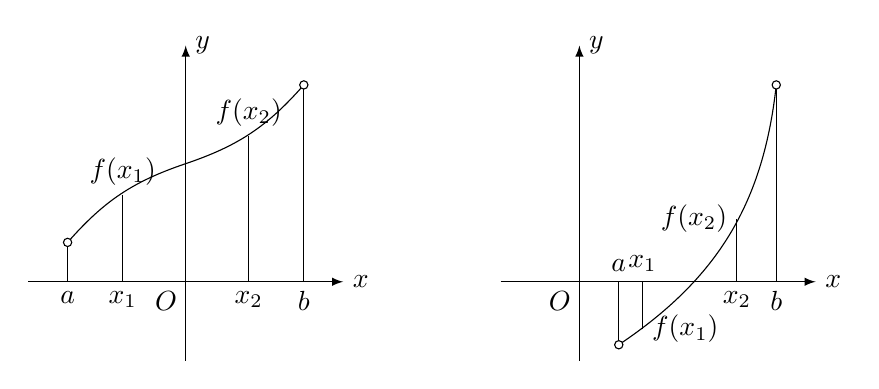
\begin{tikzpicture}[>=latex]
\begin{scope}
\draw[->](-2,0)--(2,0)node[right]{$x$};  
\draw[->](0,-1)--(0,3)node[right]{$y$};

\draw (-1.5,.5) to [bend left=15] (0,1.5) to [bend right=15] (1.5,2.5);
\draw (-1.5,.5)--(-1.5,0)node[below]{$a$};
\draw (1.5,2.5)--(1.5,0)node[below]{$b$};

\draw (-1.5,.5) [fill=white]circle(1.5pt) ;
\draw (1.5,2.5) [fill=white]circle(1.5pt) ;

\draw (-.8,1.1)node[above]{$f(x_1)$}--(-.8,0)node[below]{$x_1$};
\draw (.8,1.85)node[above]{$f(x_2)$}--(.8,0)node[below]{$x_2$};
\node at (-.25,-.25){$O$};
\end{scope}
\begin{scope}[xshift=5cm]
    \draw[->](-1,0)--(3,0)node[right]{$x$};  
\draw[->](0,-1)--(0,3)node[right]{$y$};
\draw (.5,-.8) to [bend left=-25] (2.5,2.5);
\draw (.5,-.8)--(.5,0)node[above]{$a$};
\draw (2.5,2.5)--(2.5,0)node[below]{$b$};
\node at (-.25,-.25){$O$};


\draw (.8,-.6)node[right]{$f(x_1)$}--(.8,0)node[above]{$x_1$};
\draw (2,.8)node[left]{$f(x_2)$}--(2,0)node[below]{$x_2$};
\draw (.5,-.8) [fill=white]circle(1.5pt) ;
\draw (2.5,2.5) [fill=white]circle(1.5pt) ;
\end{scope}    
\end{tikzpicture} 
